\mnDifficult
\begin{slikaDesno}[0.833]{fig/zCpi.pdf}
    \PID У систему са слике, позната је струја идеалног струјног 
генератора ${I_{\rm G} = 100\unit{\upmu A}}$ и
капацитивност $C = 1\unit{\upmu F}$, а прекидач $\Pi$ се 
може сматрати идеалним. Прекидач је отворен, осим у тренуцима 
$t = kT$, $k \in \mathbb Z$, где је $T = 1\unit{ms}$, 
када се 
\textit{краткотрајно} затвара.

\begin{enumerate}[label = (\alph*)]
    \item
    Одредити устаљене облике напона на излазу система 
    $v_{\rm I}(t)$ и струје кондензатора 
    $i_{\rm C}(t)$ према референтном смеру са слике, 
    и скицирати временске дијаграме тих сигнала.
\end{enumerate} 
\end{slikaDesno}

\begin{enumerate}[label = (\alph*)]   \setcounter{enumi}{1}
    \item Израчунати средњу снагу сигнала $v_{\rm I}(t)$,
    средњу снагу коју улаже струјни генератор, $P_{I_{\rm G}}$, и 
    средњу вредност струје кондензатора $\overline{i_{\rm C}}$. 
    
    \item
    Одредити развоје сигнала $v_{\rm I}(t)$ у комплексан и тригонометријски
    Фуријеов ред 
    на основном периоду, $V_{\rm I}[k]$, односно
    $A[k]$ и $B[k]$. 

\end{enumerate} 

\RESENJE

(а) Када је прекидач отворен, тада је $i_{\rm C} = I_{\rm G}$ па се онда на основу карактеристике кондензатора 
може писати 
\begin{equation}
    I_{\rm G} = i_{\rm C} = C \dfrac{\de v_{\rm I}}{\de t},  \label{\ID.cchar}
\end{equation}
 пошто је $v_{\rm C} = v_{\rm I}$. Одавде се онда интеграљењем обе 
стране карактеристике има 
\begin{eqnarray}
    v_{\rm I} = \dfrac{I_{\rm G}}{C} t + K, \qquad\qquad K = \const, \label{\ID.eqvin}
\end{eqnarray}
при чему је константа $K$ важећа у оквиру једног интервала док је прекидач отворен. 
Пошто се прекидач затвара у тренуцима $t = kT$ то је онда 
на основу резултата задатка \ref{ID:capID}
у тренуцима $kT^+$ кондензатор испражњен, односно је 
$v_{\rm I}(t = kT^+) = 0$. На тај начин, закључује се да је излазни напон рампа, константног нагиба 
$\dfrac{I_{\rm G}}{C} = 0,1 \unit{\dfrac{V}{ms}}$, који се у тренуцима $t = kT$ „враћа“ на вредност 0, чиме формира тестерасти облик напона 
као што је приказано на слици \ref{\ID.vi}, где је амплитуда напона
$V_{\rm m} = \dfrac{I_{\rm G} T}{C} = 100\unit{mV}$. 
%
\begin{figure}[ht!]
    \centering
        \begin{subfigure}[c]{0.45\textwidth}
            \centering
            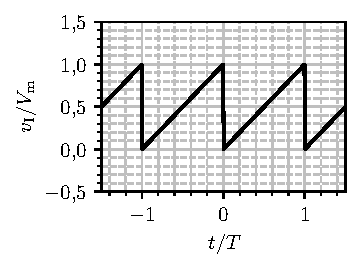
\includegraphics[scale=1]
            {fig/zCpi_vi.pdf}
            \caption{Излазни напон.}
            \label{\ID.vi}
        \end{subfigure}
        %
        \begin{subfigure}[c]{0.45\textwidth}
            \centering
            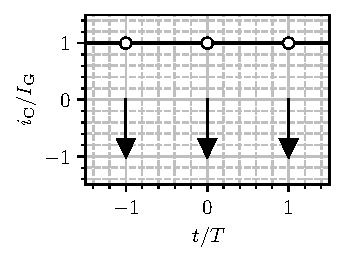
\includegraphics[scale=1]
            {fig/zCpi_ic.pdf}
            \caption{Струја кондензатора.}
            \label{\ID.ic}
        \end{subfigure}
    \caption{Тражени графици.}
\end{figure}
%
Као што је већ наглашено, струја кондензатора када је прекидач затворен износи $i_{\rm G} = I_{\rm G}$. У кратким тренуцима када је 
прекидач затворен, кондензатор се тренутно празни Дираковим импулсном струје којом приликом кроз његове прикључке протекне 
наелектрисање $Q = C V_{\rm m} = 100\unit{nC}$, што представља Дираков импулс чија је мера $-100\unit{nC}$ у тренуцима 
$kT$, што је приказано на слици \ref{\ID.ic}. Аналитички, струја кондензатора се може записати као 
\begin{eqnarray}
    i_{\rm C}(t) = I_{\rm G} ( 1 - T \III_T(t)). \label{\ID.iceqn}
\end{eqnarray}

(б) Средња снага сигнала $v_{\rm I}(t)$ може се израчунати према дефиницији у временском домену, на пример на основном периоду 
$0 < t < T$, помоћу \eqref{\ID.eqvin}, као 
\begin{equation}
    P_{v_{\rm I}} = \dfrac{1}{T} \int_{t = 0}^T v_{\rm I}^2 \, \de t  
                  = \dfrac{1}{T} \int_{t = 0}^T 
                  \left(\dfrac{I_{\rm G}}{C} t\right)^2 \, \de t  
                  = 
                  \dfrac{1}{\cancel{T}}
                  \dfrac{I_{\rm G}^2}{C^2} \dfrac{T^{\cancelto{2}{3}}}{3}
                  = 
                  \dfrac{1}{3}
                  \left(
                    \dfrac{I_{\rm G} T}{C }
                  \right)^2
                  = \dfrac{1}{300} \unit{V^2}
\end{equation}

(б) 
Снага струјног генератора може се израчунати помоћу средње вредности напона на излазу као 
\begin{equation}
    P_{I_{\rm G}} = \overline{I_{\rm G} \cdot v_{\rm I}} = I_{\rm G} \cdot \overline{v_{\rm I}} = \dfrac{I_{\rm G} V_{\rm m}}{2} = 5\unit{\upmu W}.
\end{equation}

Средња вредност струје кондензатора може се наћи директно, или усредњавањем на основу карактеристике\footnote{
    Добијени резултат да је у периодичном режиму средња струја кондензатора $\overline{i_C} = 0$, представља 
    и еквивалентан исказ да је у устаљеном режиму једносмерна компонента струје кондензатора равна нули, еквивалентно 
    кондензатор је отворена веза за сталне струје. Овај исказ такође има велику примену у Енергетској електроници 
    где је познат и под именом ампер--секунд баланс. 
} 
\begin{equation}
    \overline{i_{\rm C}} = \dfrac{1}{T}\int_{t_0}^{t_0 + T} i_{\rm C} \de t = 
    \dfrac{C}{T} \underbrace{ \left( v(t - T) - v(t) \right) }_{=0,\ \text{због периодичности}} = 0.
\end{equation}

(в) Тражени спектар може се одредити полазећи од спектра струје кондензатора, а који се одређује на основу израза 
\eqref{\ID.iceqn}, одакле се има
\begin{eqnarray}
    I_C[k] &=& \FS{ i_C(t) } = \FS{ I_{\rm G} ( 1 - T \III_T(t)) } \\
    &=& 
    I_{\rm G} \left( 
    \FS{1} - T \underbrace{\FS{\III_T(t)}}_{\text{Задатак \refz{dirak_povorka}}} 
    \right)
    = I_{\rm G}(\updelta[k] - 1). 
\end{eqnarray}
Пошто важи карактеристика кондензатора \eqref{\ID.cchar}, за одговарајуће спектре ће важити\footnote{Применом својства 
дејства Фуријеовог реда на интеграл: $\int \mapsto \cdot \dfrac{1}{\jj k \upomega_{\rm F}}$. }
\begin{eqnarray}
    V_{\rm I}[k] = \dfrac{1}{\jj k \upomega_0 C} I_{C}[k] = 
    - \dfrac{I_{\rm G}}{\jj k \upomega_0 C}, \qquad \upomega_0 = \dfrac{2\uppi}{T} \qquad
    \text{осим за $k = 0$.}
\end{eqnarray}
Члан $V_{\rm I}[0]$ се може одредити као средња вредност сигнала, односно $V_{\rm I}[0] = \dfrac{V_{\rm m}}{2}$, па је коначно 
\begin{equation}
    V_{\rm I}[k] = 
    \begin{cases}
        \dfrac{I_{\rm G} T}{2C} &,  k = 0 \\[4mm]
        \dfrac{\jj I_{\rm G}}{k \upomega_0 C} &, k \neq 0
    \end{cases}
\end{equation}
Примећујемо да је добијени спектар чисто непаран (са изузетком члана $k=0$) па ће све косинусне компоненте 
сигнала бити $A[k > 0] = 0$, док се синусне компоненте могу наћи као\footnote{Видети и додатак \ref{d:CTFS}.}
\begin{eqnarray}
    B[k > 0] = -2\, \Im{V_{\rm I}[k]} = - \dfrac{2 I_{\rm G}}{k \upomega_0 C},
\end{eqnarray}
па је коначно 
$
    v_{\rm I}(t) = \dfrac{I_{\rm G} T}{2 C } 
    - 
    \sum_{k = 1}^{\infty}
    \dfrac{2 I_{\rm G}}{k \upomega_0 C} \sin(\upomega_0 t)$,
што се може преуредити у једноставнији облик 
\begin{eqnarray}
    v_{\rm I}
    = 
    \dfrac{I_{\rm G} T}{C} 
    \left(
    \dfrac{1}{2}
    - 
    \sum_{k = 1}^{\infty} 
    \dfrac{1}{ k \uppi} \sin(k \upomega_0 t)
    \right)
\end{eqnarray}
